\documentclass{article}
\usepackage{graphicx}
\usepackage{mathtools}
\usepackage{xfrac}
\usepackage{amsmath, amssymb}
\usepackage{listings}
\usepackage{float}
\usepackage{wrapfig}
\usepackage{tikz}
\usepackage{fullpage}
\usepackage{hyperref}
\usepackage{mathalpha}
\usepackage{tikz}
\usepackage{cite}
\usepackage{amsthm}
\usepackage{natbib}

\newtheorem{theorem}{Proposition}[section]
\newtheorem{corollary}{Corollary}[theorem]
\newtheorem{lemma}[theorem]{Lemma}

\theoremstyle{definition}
\newtheorem{definition}{Definition}[section]

\theoremstyle{remark}
\newtheorem*{remark}{Remark}
\newtheorem*{example}{Example}
\newtheorem*{notation}{Notation}

\title{Computational Simulation: Numerical Methods\\Assignment 3}
\author{David Lawton\\22337087}
\date{20th Oct. 2024.}

\begin{document}

\maketitle

\tableofcontents

\section{Introduction}
This report details the 3rd assignment of Computer Simulation I. The assignment entails finding the numerical solution of a given ordinary differential equation (ODE) using several methods, and comparing the results. The given ODE is
\begin{equation}
    \label{eq: ODE}
    f(x, t) = \frac{dx}{dt} = (1+t)x + 1 - 3t + t^2 
\end{equation} 
The process involves visualising the solution using the \textit{direction field} of the ODE, and then solving the ODE using the \textit{Euler method}, the \textit{Improved Euler method}, and the \textit{4th order Runge-Kutta method}. The starting value $x_0$ of the numerical integration is $x_0 = 0.0655$ (which is near the \textit{critical point} $x=0.065923$), and the behaviour was analysed on varying time-scales. \\

\section{Background \& Theory}

The first step in solving the ODE is to visualise the solution using the \textit{direction field}. The direction field is a field of vectors that take direction and relative magnitude from the value of $\frac{dx}{dt}$ at each of an array of points, each vector $\vec{v}$ at a point $(x_i, t_i)$ is given by

\begin{equation}
    v_x = 1\cdot C \quad v_t = f(x_i, t_i)\cdot C
\end{equation}

where C is a scaling constant, and $v_x, v_t$ are the components of the vector in the $x$ and $t$ directions respectively. The direction field of the ODE in Eq. \ref{eq: ODE} is shown in Fig. \ref{fig: direction field}. \\

\begin{figure}[H]
    \centering
    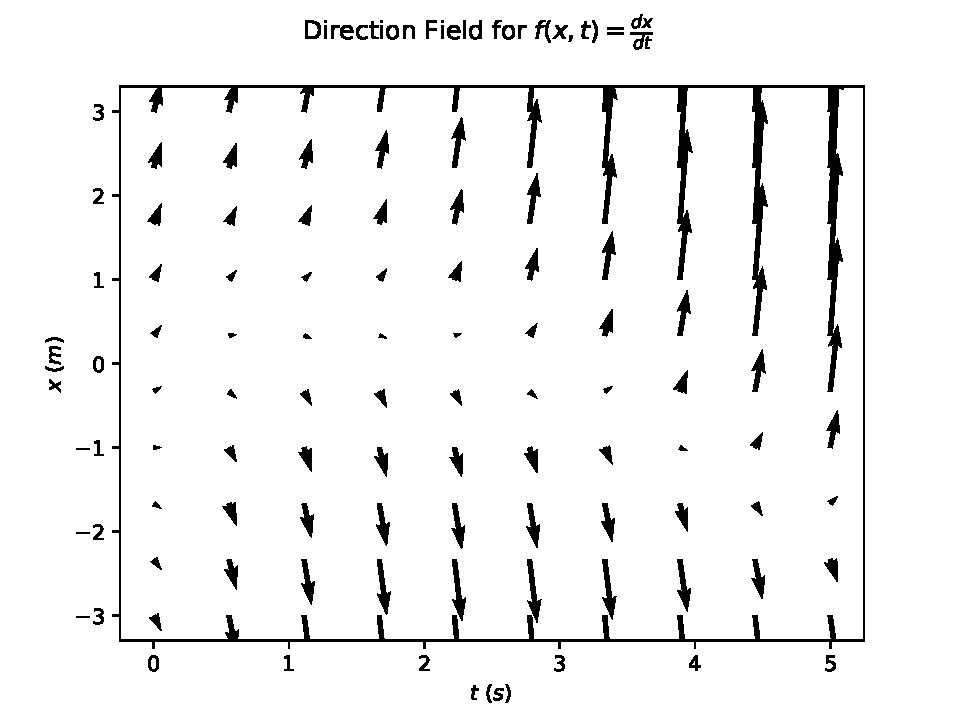
\includegraphics[width=0.7\textwidth]{/home/dj-lawton/Documents/Junior Sophister/Computer Simulation/Numerical Methods/Assignment 3/Direction_Field.pdf}
    \caption{\label{fig: direction field}The direction field of the ODE defined in Eq. \ref{eq: ODE}, note the region along which the vectors are small, the field diverges away from this line.}
\end{figure}

\indent The three methods of numerical integration we used in this assignment are the \textit{Euler method}, the \textit{Improved Euler method}, and the \textit{4th order Runge-Kutta method}.

\subsection{Euler Method}
The Euler method is the simplest method of numerical integration, and is given by the iterative formula

\begin{equation}
    x_{i+1} = x_i + \frac{dx}{dt}\cdot \Delta t
\end{equation}

one chooses the value of $x_0$ and then iterates the formula to find the value of $x$ at each time step. Euler's method approximates the curve in $[t_i, t_{i+1}]$ by a straight line of slope $\frac{dx}{dt}|_{x_i, t_i}$. The error of this method is of order $\Delta t^2$ locally and $\Delta t$ globally.(\cite{2020Euler})\\

\subsection{Improved Euler Method}
The Improved Euler method is a modified version of the Euler method that estimates the endpoint of the curve in $[t_i, t_{i+1}]$ using Euler's method and averages the slope at these two points, as say $\tilde{f}$. It then executes the iterative method
\begin{equation}
    x_{i+1} = x_i + \tilde{f}\cdot \Delta t \quad \text{where,} \quad \tilde{f} = \frac{1}{2}\left(f(x_i, t_i) + f(x_i + f(x_i, t_i)\cdot \Delta t, t_i+\Delta t)\right)
\end{equation}
This error of this method is locally of order $\Delta t^3$ and globally of order $\Delta t^2$.(\cite{2020Improved})\\

\subsection{4th Order Runge-Kutta Method}
The 4th of two points like the improved Euler method, slopes of four points, and a weighted average, to estimate the value of $x_{i+1}$. The iterative formula is given by
\begin{equation}
    x_{i+1} = x_i + \frac{1}{6}(k_1 + 2k_2 + 2k_3 + k_4)\cdot \Delta t
\end{equation}
where $k_1, k_2, k_3, k_4$ are given by
\begin{align*}
    k_1 &= f(x_i, t_i) \\
    k_2 &= f(x_i + \frac{1}{2}k_1\cdot \Delta t, t_i + \frac{1}{2}\Delta t) \\
    k_3 &= f(x_i + \frac{1}{2}k_2\cdot \Delta t, t_i + \frac{1}{2}\Delta t) \\
    k_4 &= f(x_i + k_3\cdot \Delta t, t_i + \Delta t)
\end{align*}
This is the most accurate of the three methods, as the local error is of order $\Delta t^5$ and the global error is of order $\Delta t^4$.

\section{Results}
Our first result emerges from our use of the Euler method and illustrates its inaccuracy.
\begin{figure}[H]
    \centering
    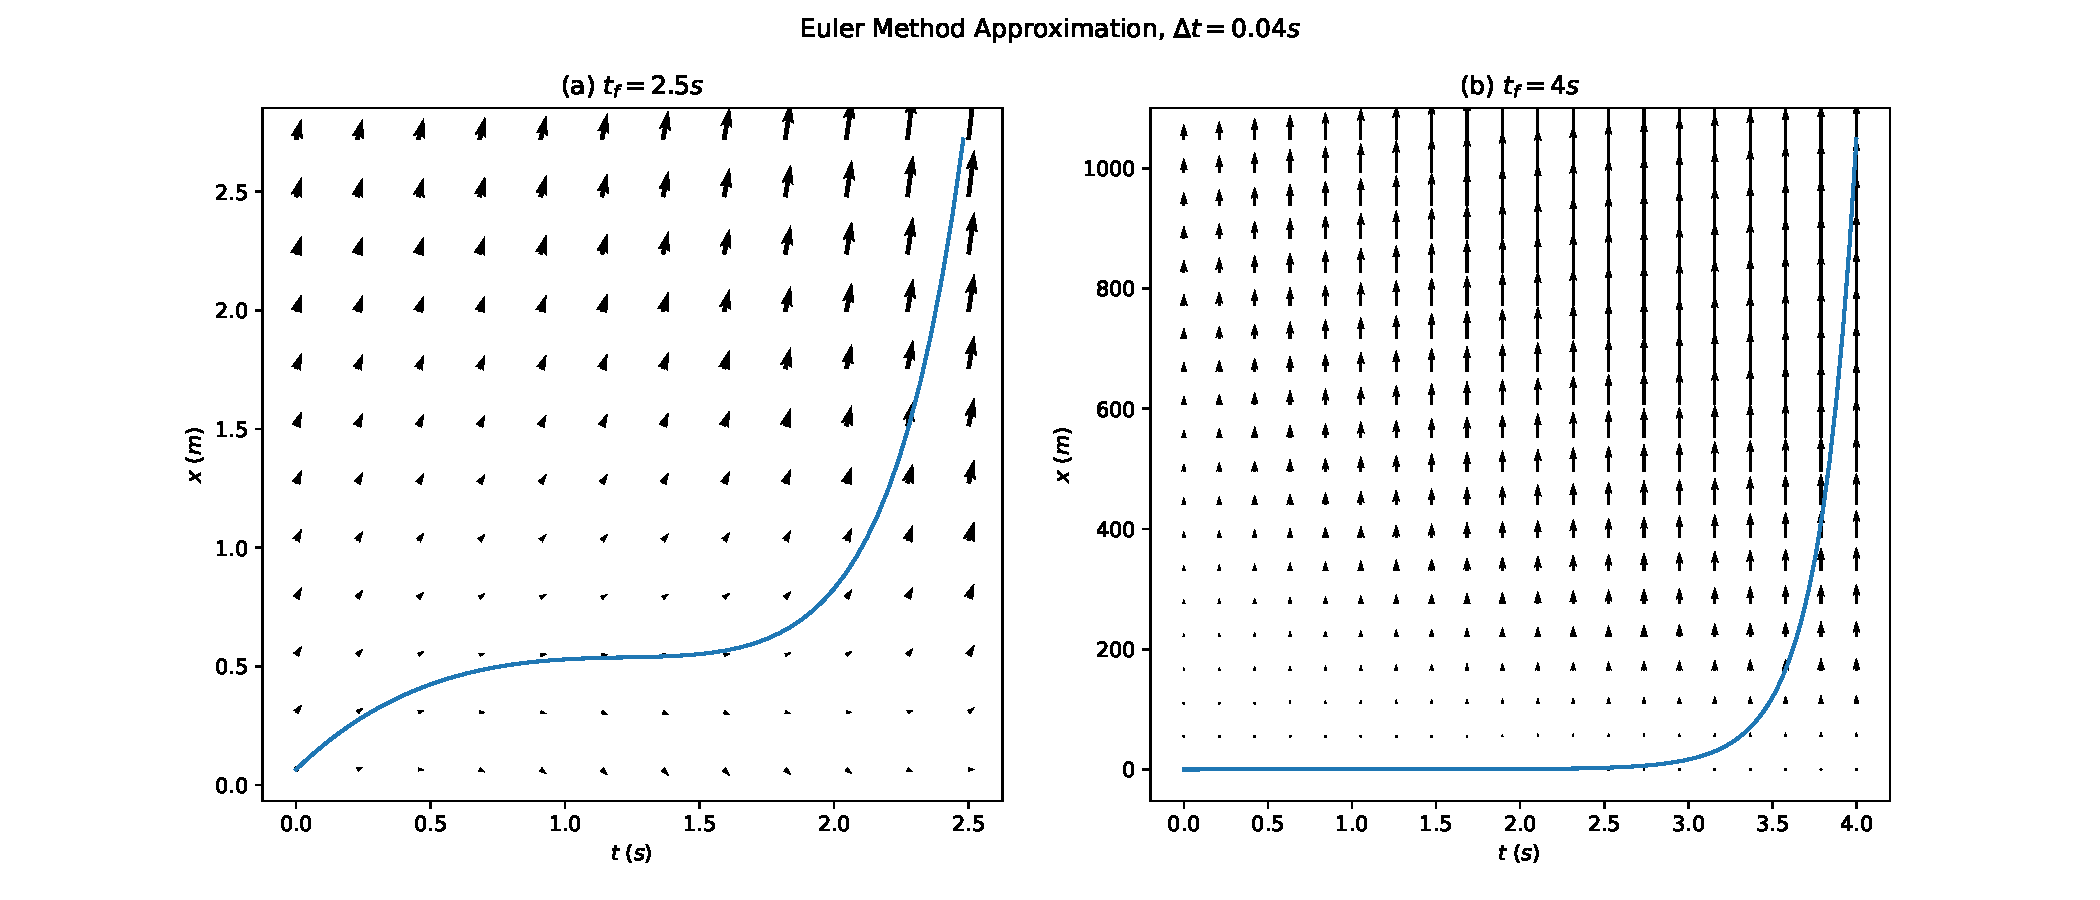
\includegraphics[width=0.9\textwidth]{/home/dj-lawton/Documents/Junior Sophister/Computer Simulation/Numerical Methods/Assignment 3/Euler_Method_Approximation_0.04.pdf}
    \caption{\label{fig: Euler method 0.04} The approximation of the ODE in Eq. \ref{eq: ODE}, using the Euler method with $\Delta t = 0.04$. The approximation is clearly poor, as the curve diverges to $+\infty$, when it starts below the critical point, and should diverge to $-\infty$.}
\end{figure}
While the initial point $x_0=0.0655$ is below the critical point $x_c=0.065923\dots$, and should diverge to $-\infty$, the Euler method approximation of the solution diverges to $+\infty$ in Fig. \ref{fig: Euler method 0.04}.\\
\indent Next we observe the behaviour of the higher order methods used. 

\begin{figure}[H]
    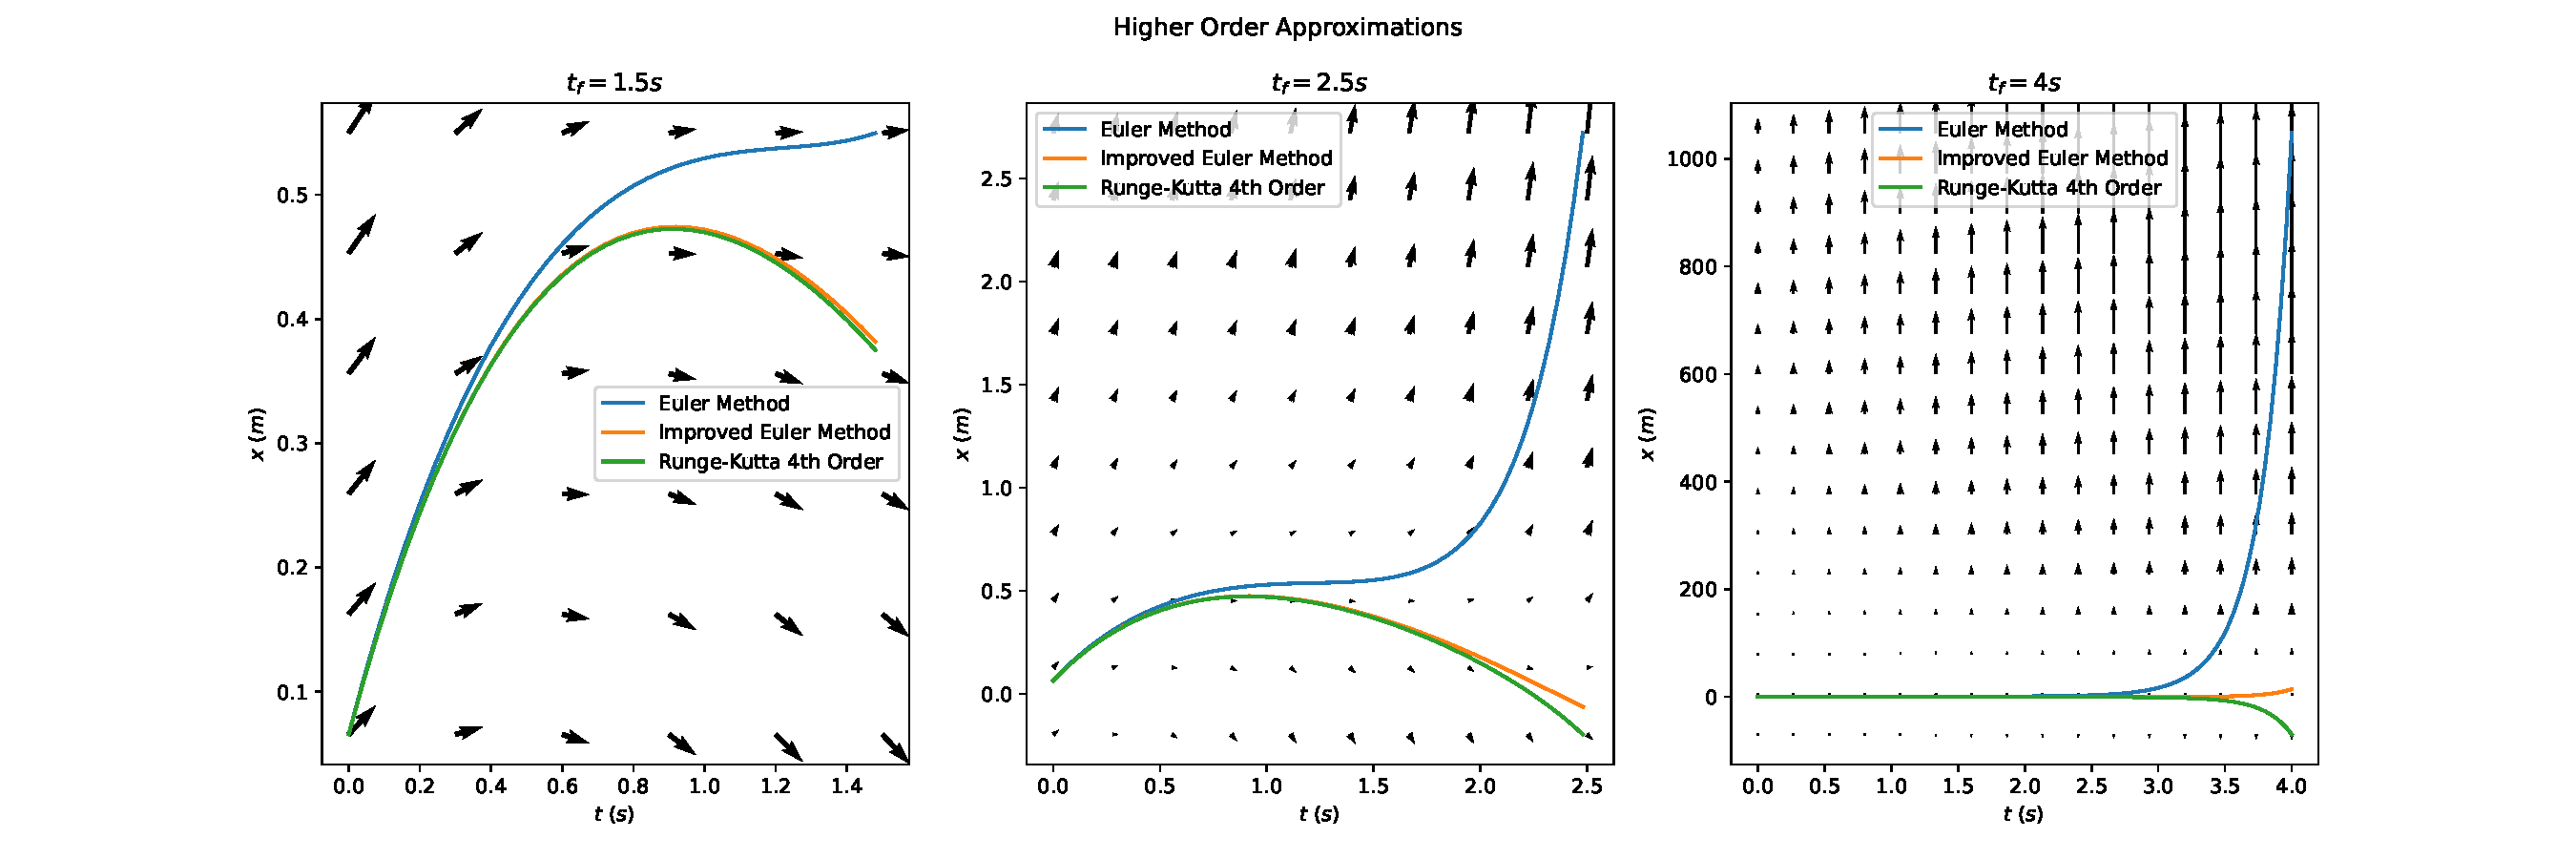
\includegraphics[width=1\textwidth]{/home/dj-lawton/Documents/Junior Sophister/Computer Simulation/Numerical Methods/Assignment 3/Higher_Order_Approximations_0.04.pdf}
    \caption{\label{fig: Higher order methods 0.04} The approximation of the ODE in Eq. \ref{eq: ODE}, using the Improved Euler method and the 4th order Runge-Kutta method with $\Delta t = 0.04$, compared to the simple Euler method. Both of the higher order methods approximate the solution better than the simple Euler method, but the 4th order Runge-Kutta method is the most accurate, as it does begin to diverge downwards.} 
\end{figure}
In Fig. \ref{fig: Higher order methods 0.04}, on the small scale, each of the methods seems to follow the direction field well. However, the large scale behaviour, versus expectations, also indicates the accuracy of each method. The 4th order Runge-Kutta method can be seen as the most accurate, as it diverges downwards, as expected, unlike the other two.\\
\indent It follows to alter the step-size to see how it affects the accuracy. We reduce the step-size to $\Delta t = 0.02$, while keeping $x_0=0.0655$ the same, outputting the following results.
\begin{figure}[H]
    \centering
    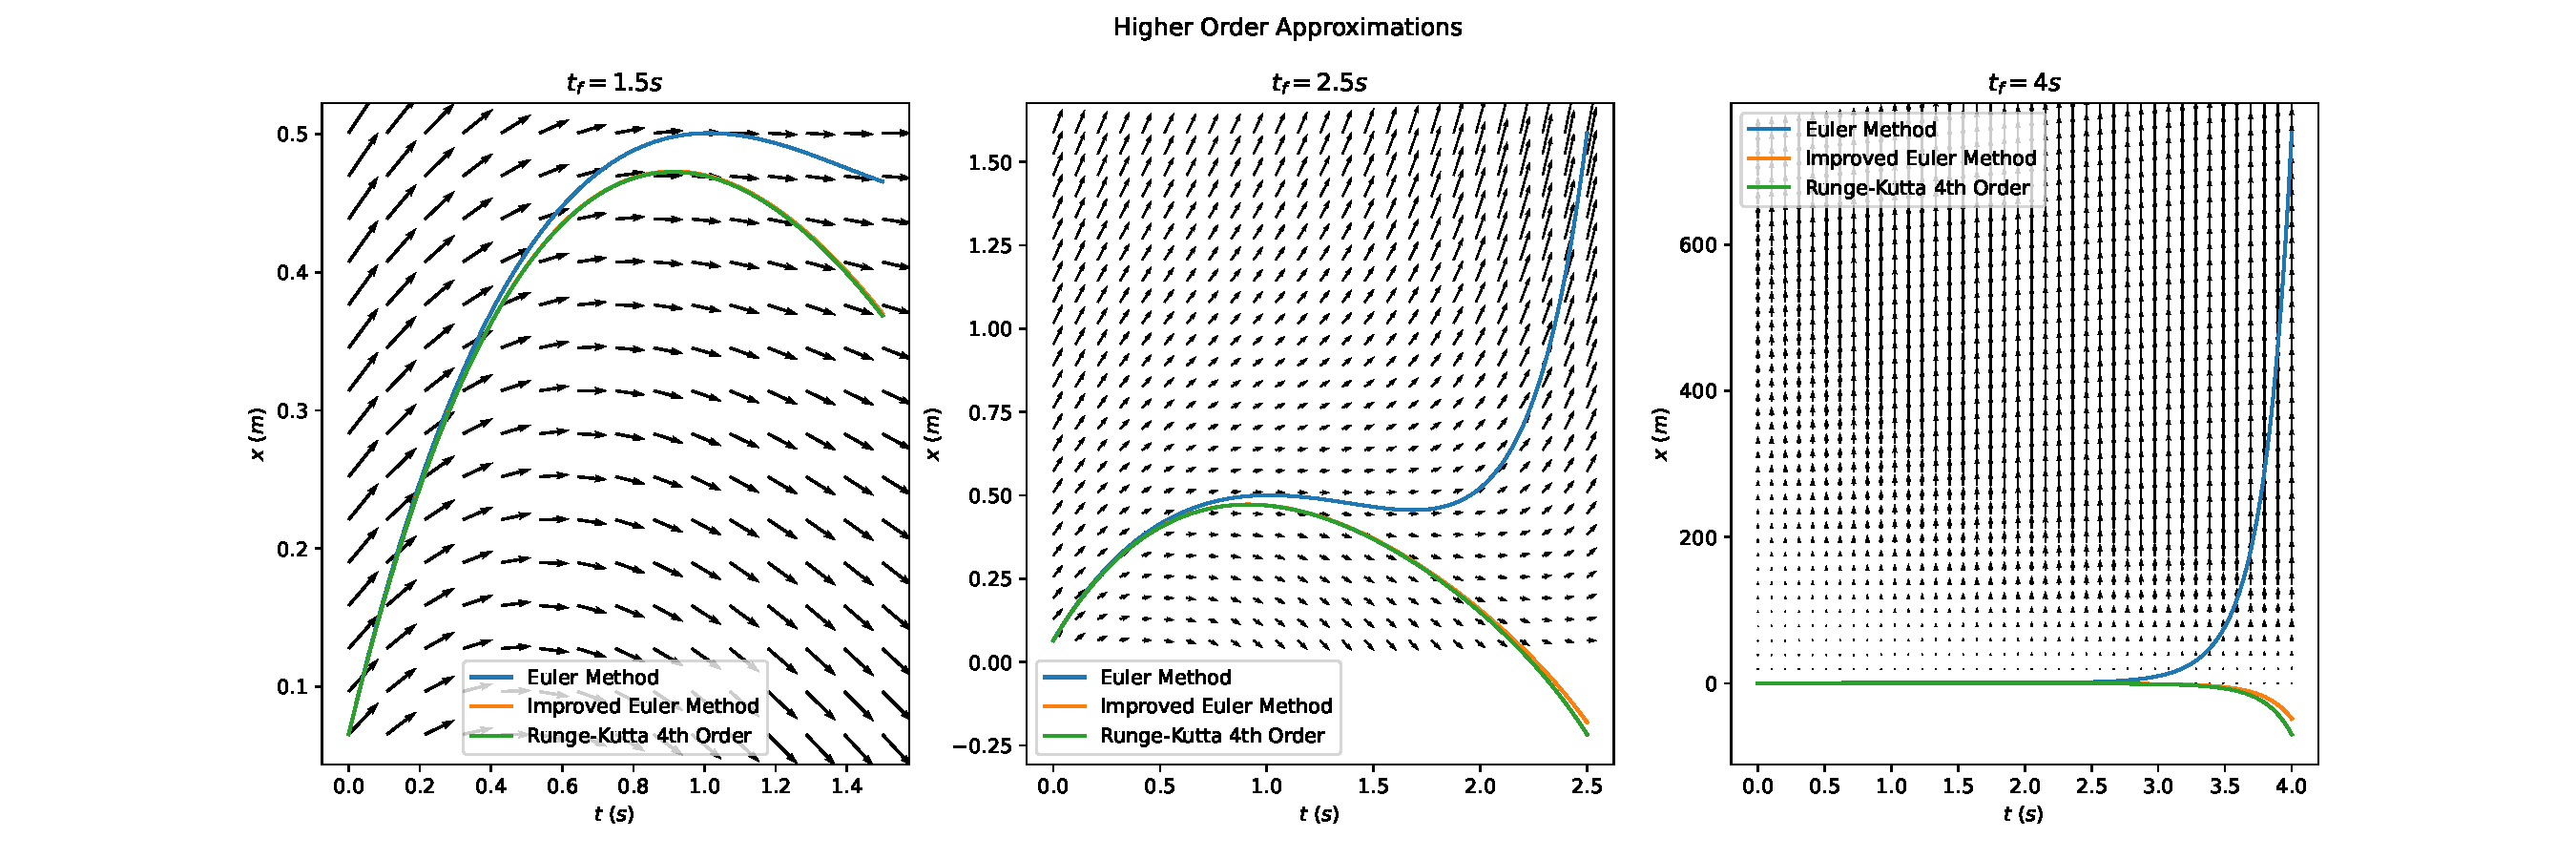
\includegraphics[width=\textwidth]{/home/dj-lawton/Documents/Junior Sophister/Computer Simulation/Numerical Methods/Assignment 3/Higher_Order_Approximations_0.02.pdf}
    \caption{\label{fig: Higher order methods 0.02} }
\end{figure}
The improvement in accuracy of the Euler method is clear in Fig. \ref{fig: Higher order methods 0.02}, with a little more downward curvature before divergence, although it still diverges upwards. The Improved Euler approximation illustrates best the improvement in accuracy as it now starts to diverge downward as $t$ gets larger, as expected. The difference in accuracy of the 4th order Runge-Kutta method is less clear, due to the smaller change relative to the other two.\\
\indent We can conclude from this the benefit of using higher order methods. It is evident that the higher order approximations, especially the 4th order Runge-Kutta, require far fewer steps to achieve an accurate approximation, and are thus less prone to rounding errors in high precision calculations. The reduction in steps also reduces the computational cost of the calculation, making it more efficient.\\

\section{Appendix}
Code used in this assignment is attached, but can also be found at \url{https://github.com/DavidLawton04/MuchStuff/tree/62c15d25ead9639dfba68440ad189b285fffb30a/Junior%20Sophister/Computer%20Simulation/Numerical%20Methods/Assignment%203}

\bibliographystyle{plainnat}
\bibliography{references}
\end{document}